


\begin{center}
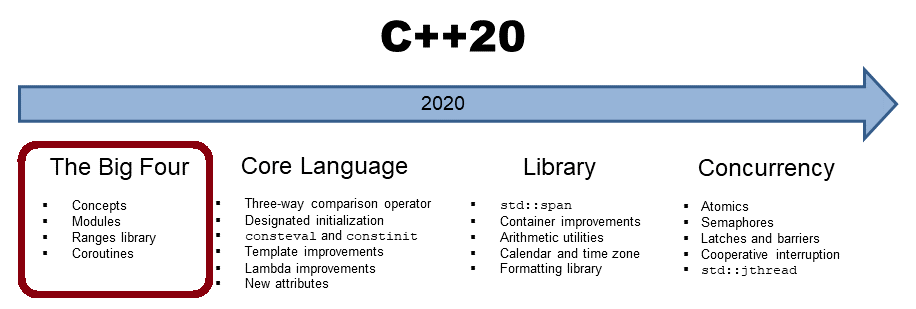
\includegraphics[width=1.0\textwidth]{content/2/chapter3/images/2.png}\\
每一个特性都会改变使用C++的方式。
\end{center}

\subsubsubsection{3.1.1\hspace{0.2cm}概念}

使用模板的泛型编程,使其能够定义可用于各种类型的函数和类。因此,使用错误类型实例化模板的情况并不少见,因此会看到长达数页的编译错误,而这个问题可以通过概念解决。概念可编写编译器检查模板参数的需求,并彻底改变开发者思考和编写泛型代码的方式:

\begin{itemize}
\item 
模板参数的需求成为公共接口的一部分。

\item 
函数的重载或类模板的特化可以基于概念。

\item 
因为编译器会根据给定的模板参数检查已定义的模板形参需求,所以可以得到了更明确的错误消息。
\end{itemize}

这还没完。

\begin{itemize}
\item 
开发者可以使用预定义的概念,也可以自定义概念。

\item 
auto和概念的用法统一,可以用概念来代替auto。

\item 
若函数声明使用了概念,则自动成为函数模板。编写函数模板就像编写函数一样简单。
\end{itemize}

下面的代码片段演示了概念Integral的定义和使用:

\begin{lstlisting}[style=styleCXX]
template <typename T>
concept Integral = std::is_integral<T>::value;

Integral auto gcd(Integral auto a, Integral auto b) {
	if( b == 0 ) return a;
	else return gcd(b, a % b);
}
\end{lstlisting}

Integral概念从其类型参数T中要求std::is\_integral<T>::value为true。std::is\_integral<T>::value来自\href{https://en.cppreference.com/w/cpp/header/type_traits}{类型特征库},在编译时检查T是否为整数。若std::is\_integral<T>::value为true,则一切正常;否则,将会看到相应的编译时错误。

gcd算法基于\href{https://en.wikipedia.org/wiki/Euclid}{Euclidean}确定最大公约数,代码使用缩写函数模板语法来定义gcd。这里,gcd要求参数和返回类型支持Integral概念。换句话说,gcd是一种对其参数和返回值类型有要求的函数模板。

下面是语义等效的gcd算法,使用了require子句。

\begin{lstlisting}[style=styleCXX]
template<typename T>
requires Integral<T>
T gcd(T a, T b) {
	if( b == 0 ) return a;
	else return gcd(b, a % b);
}
\end{lstlisting}

require子句声明了对gcd参数类型的要求。

\subsubsubsection{3.1.2\hspace{0.2cm}模块}

模块的作用有很多:

\begin{itemize}
\item 
更快的编译时间

\item 
减少宏定义

\item 
表达代码的逻辑结构

\item 
淘汰头文件

\item 
摆脱宏替换
\end{itemize}

这是一个简单的数学模块:

\begin{lstlisting}[style=styleCXX]
export module math;

export int add(int fir, int sec) {
  return fir + sec;
}
\end{lstlisting}

表达式会导出模块math(第1行)是模块声明,将export放在函数add之前(第3行)导出函数。现在,可以使用它了。

\begin{lstlisting}[style=styleCXX]
import math;

int main() {
	add(2000, 20);
}
\end{lstlisting}

表达式import math导入math模块,并使导出名在当前作用域中可见。

\subsubsubsection{3.1.3\hspace{0.2cm}范围库}

范围库支持的算法有如下特征

\begin{itemize}
\item 
可直接在容器上操作,不需要迭代器来指定范围

\item 
可以延迟求值

\item 
可以组合
\end{itemize}

简而言之:范围库支持函数模式。

下面的例子展示了如何组合管道操作符。

\begin{lstlisting}[style=styleCXX]
int main() {
	std::vector<int> ints{0, 1, 2, 3, 4, 5};
	auto even = [](int i){ return i % 2 == 0; };
	auto square = [](int i) { return i * i; };
	
	for (int i : ints | std::views::filter(even) |
						std::views::transform(square)) {
		std::cout << i << ' '; // 0 4 16
	}
}
\end{lstlisting}

even(第3行)是Lambda表达式,若参数i是偶数,则返回true。Lambda表达式square(第4行)将计算参数i为的平方。第6行和第7行演示了函数组合,必须从左到右阅读:for (int i: ints | std::views::filter(even) | std::views::transform(square))。对int类型的每个元素应用偶数过滤器,并将每个剩余元素计算其平方值。若熟悉函数式编程,那么这段代码看起来就很容易。

\subsubsubsection{3.1.4\hspace{0.2cm}协程}

协程是可以在保持其状态的同时挂起并稍后恢复的函数,协程是编写事件驱动应用程序的一种方法,通常也用于协作多任务处理。事件驱动的应用程序可以是模拟、游戏、服务器、UI,甚至算法。

C++20没有提供协程库,而提供了一个实现协程的框架。该框架由20多个函数组成,其中一些必须实现,一些可选实现。因此,可以根据自己的需要定制协程。

下面的代码片段使用生成器创建无限的数据流。本章协程提供了生成器实现的版本。

\begin{lstlisting}[style=styleCXX]
Generator<int> getNext(int start = 0, int step = 1){
	auto value = start;
	while (true) {
		co_yield value;
		value += step;
	}
}

int main() {
	
	std::cout << '\n';
	
	std::cout << "getNext():";
	auto gen1 = getNext();
	for (int i = 0; i <= 10; ++i) {
		gen1.next();
		std::cout << " " << gen1.getValue();
	}
	
	std::cout << "\n\n";
	
	std::cout << "getNext(100, -10):";
	auto gen2 = getNext(100, -10);
	for (int i = 0; i <= 20; ++i) {
		gen2.next();
		std::cout << " " << gen2.getValue();
	}
	
	std::cout << "\n";

}
\end{lstlisting}

因为co\_yield关键字,所以getNext是协程。这里有一个无限循环,会在co\_yield处返回值(第4行),在next(第16行和第25行)处恢复运行,然后调用getValue获取值。在getNext调用返回之后,协程再次暂停,直到下一次调用next。在这个例子中有一个迷:getNext函数的返回值Generator<int>。这就开始复杂了,我将在协程部分中深入地进行讲解。

\begin{center}
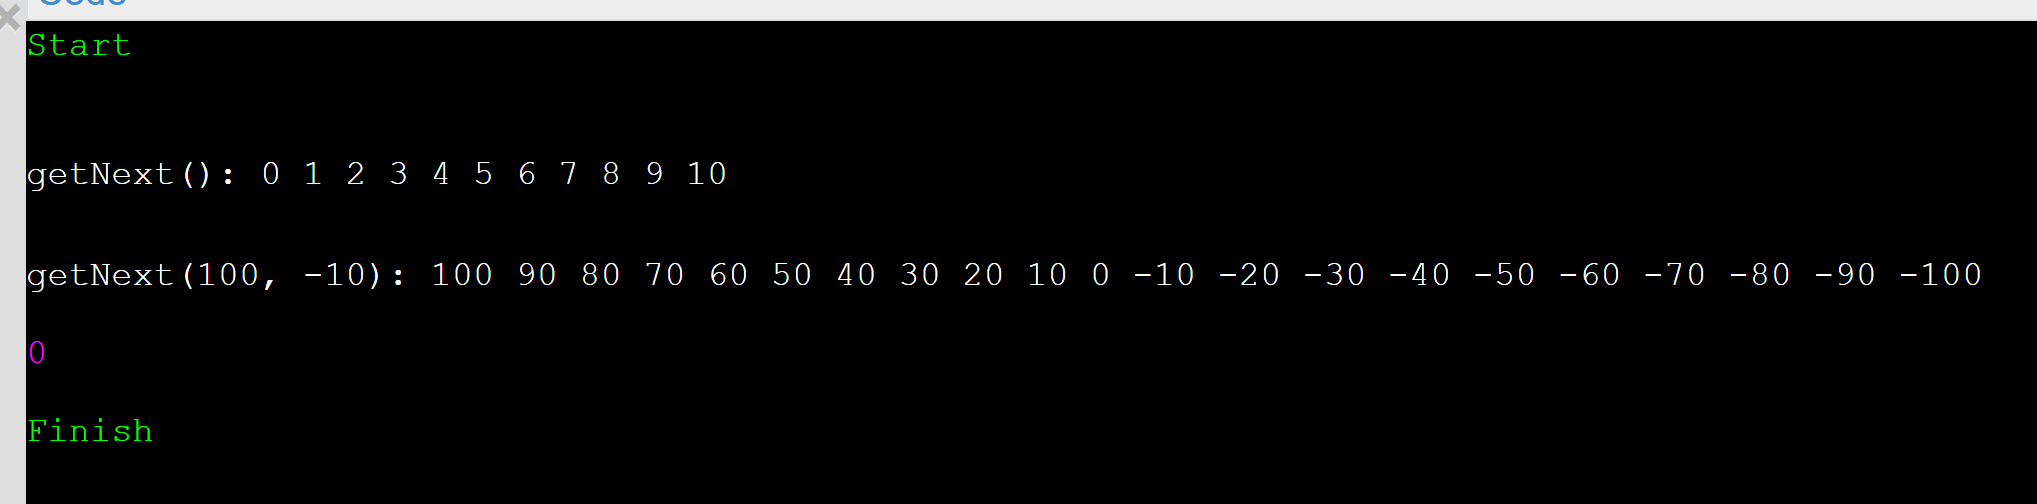
\includegraphics[width=1.0\textwidth]{content/2/chapter3/images/3.png}\\
\end{center}















